\section{Methodology}



This mutation framework is specifically designed for Scala and relies on Scala compiler library to give us access to an intermediate representation of the program. Since the proposed mutation framework is expected to be extensible, we have made it as flexible as possible with respect to mutation locations and operators. This tool comes with a configuration object that maintains the requirements of the user.  To enable a configuration, for example Spark compatible mutation, a user can submit that configuration to the framework. These configurations are then accessed later in the process of mutation to find mutation candidates location. Configurations include: 
\begin{itemize}
\item Candidate operators for mutations
\item Set of possible mutation operators
\item Preset Mutation Location for Spark
\item Probabilistic model for mutation location 
\end{itemize}

Once the configurations are supplied to the framework, it starts the step by step procedure to apply mutations on the user given programs. It starts of by a first generating the AST representation of the given source. This AST is then traversed to find the mutation locations. When such location is retrieved, an appropriate mutation is then applied by transforming the current AST. This newly transformed mutated AST is translated into a source code so that a user can identify the mutation when a test fails. These steps are also illustrated in Figure~\ref{flow}. In the later sections, we will go into the detail for each of the 4 steps of mutating a program.

\subsection{AST Generation}
This framework applies mutation on the Abstract syntax tree representation of the program. The decision on choosing AST for mutation application is based on the requirement that we want the mutated program to be syntactically correct. AST gives this framework access to the exact operators and functions that are needed to be mutated while keeping the program syntax correct. 
In the first step of this pipeline, we generate the AST of the every module in the user given project. To generate AST of  a Scala class we used Scala compiler library. This library produces the AST which is similar to the one generated when a program is compiled. A portion of  AST of a program is also shown in Figure~\ref{ast}.  One hurdle that we faced here is that this AST generated is immutable. Since in the later steps we have to mutate the AST , a mutable version of this AST is required to transform it as needed. Manually cloning of this AST is also not feasible. To get a mutable AST from Scala compiler plugin, we used the  abstract syntax tree transformation module. This allows us to rewrite and make changes to the nodes in AST. 

\begin{figure}[H]
\centering
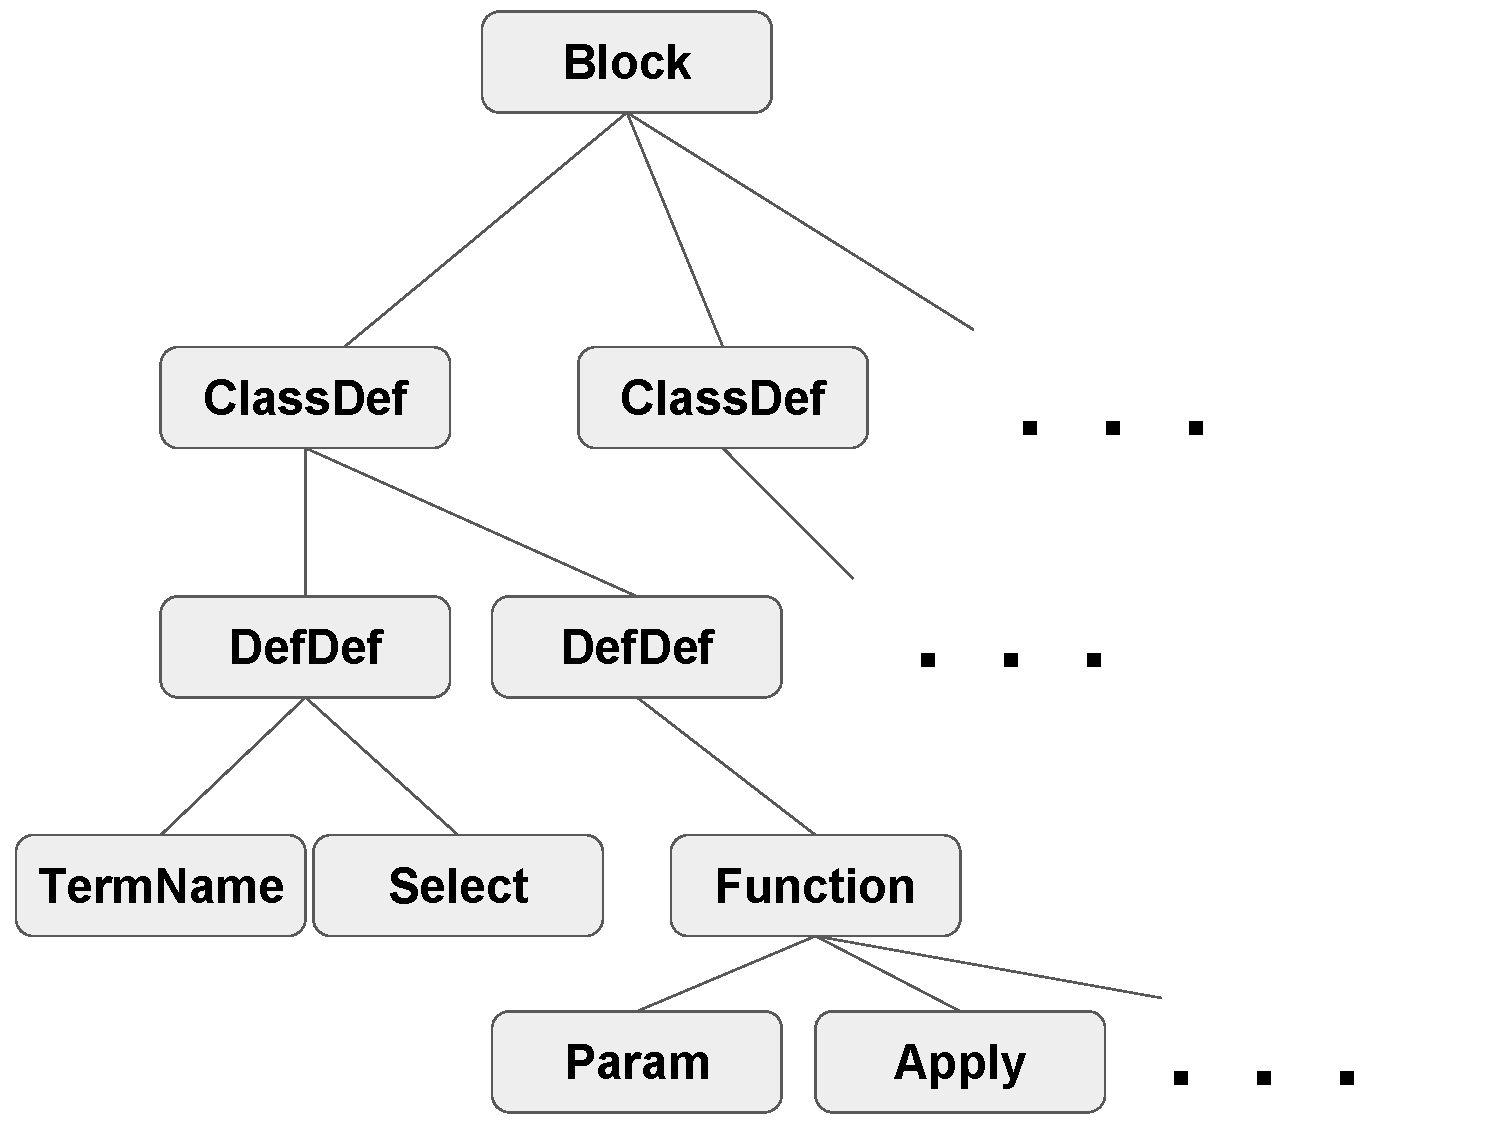
\includegraphics[width=0.4\textwidth]{image/ast}
 \caption{A sample AST with some nodes }
        \label{ast}
\end{figure}


\subsection{Tree Matching}
In this tool, we are targeting operators that are user defined and provided through the user configurations. To introduce mutations in a program, the AST of that program needs to be traversed in order to find appropriate locations (specifically nodes) where a mutation can be applied. We apply depth first search on the generated AST to find the operators and code location where the mutation should be applied. Starting with the module, this framework explores the subtree under every AST node and eventually reaches a node which is a mutation candidate. These candidates nodes are found using pattern and/or type matching of Scala. For arithmetic and boolean operators such  \texttt{+,-,>} etc, we looked for a pattern like this 
 \texttt{(SELECt(..., TERMNAME(\$plus))}  in each subtree. This search strategy works well and finds all the usage of the user defined operators that may possibly be mutated.

If a user configure the framework to work with Spark program, then we are only interested in mutating the program code that is used as closure and supplied to transformation operators. This choice of mutation location only mutates the Spark?s transformation code rather the Spark internals since the goal is to mutate that user written application. Such user written closures are detected using the pattern  \texttt{(Function(..., TERMNAME))}. This pattern cover all the UDFs in the given program and thus localize the user written code. If an AST node is found with such signature, the subtree under that node will be flagged as mutation target. By default the whole AST is flagged as non-mutation target. The implementation of this approach is flexible and can be used to localize any kind of code fragments but as of now only binary, arithmetic and UDFs based patterns are enabled. 
\subsection{Mutation Insertion}
At this point, we already have the node that is needed to be mutated. We apply the transformation as given in the user defined configuration file and replace the node with the newly generated mutated node. 
\begin{center}
\texttt{Select(b,t1,newTermName("\$minus"))-> Select(b,t1,newTermName("\$plus"))}
\end{center}
After this transformation the framework increment a newer version of the program that contains this mutant. At the end of the whole mutation process, for every mutant applied to the program, a new mutated program version would be generated. Since the mutation locations and operators are user defined, if the operator on the node is marked as the one not to be mutated then we skip the current node and move to next possible mutation location. Furthermore, in the same step we also apply the probabilistic mutation. A user defined probabilistic model is used to make a decision on whether to apply the mutation or not at the mutation candidate node. By default this model is defined in configuration as uniform distribution between 0-1.
\subsection{Refactoring and Source Code Generation}
Once we insert a mutation, the transformed AST is forwarded to refactoring and code generation module of the framework.  Since we want to keep the source code of the mutated program, we use Scala reflect library that transforms the AST into a readable source code. Keeping source code of the mutated version of the program is necessary because a user may want to compare mutation location with a fault inducing location identified from a fault localization tool. 
Converting an AST into source code is not a perfect process. The conversion from a source code into AST might lead to loss of information about the code which consequently lead to incomplete code generation when converting to source code. We rely on Scala compiler library to generate AST and to keep full information of the source code to recover it back when required. Unfortunately, the library loses information which makes is harder to generate a complete and compilable source code. In most of the cases that we observed in our subject programs, the generated source required minor cosmetic changes to make is compilable. We apply these refactoring to make the code compilable. The most frequent refactoring is the removal of  \texttt{BLOCK}  node and re-introducing package information.  \texttt{BLOCK}  node refactoring is needed because Scala compiler plugin assumes that every AST is part of a  \texttt{BLOCK}  node. The use of  \texttt{BLOCK}  node is helpful if we have multiple classes within the same file e.g  \texttt{BLOCK([class1, class2])}. The generated code  also contains the code for those  \texttt{BLOCK}  nodes. We refactor the program to remove these code fragments and transform the code into a compilable Scala code. The readable mutated code is saved into a file under the respective directory which can be built and run. 



